\documentclass{beamer}

\usepackage[utf8]{inputenc}
\usepackage{default}
\usepackage[utf8]{inputenc}
% \usepackage{fullpage} 
\usepackage{verbatim}
\usepackage{multirow}
\usepackage{marginnote}
% \setcounter{tocdepth}{4}
% \usepackage{tocloft}
\usepackage{tikz}
\usetikzlibrary{arrows,fit,positioning}


% \usepackage{tocstyle}
\usepackage[nottoc,numbib]{tocbibind} %https://tex.stackexchange.com/questions/8458/making-the-bibliography-appear-in-the-table-of-contents
\settocbibname{References}

\usepackage{csquotes}




\title{Ethereum, Smart-contracts, Swarm, Web 3.0}
\author{Viktor Tron and Aron Fischer}

\AtBeginSection[]
{
\begin{frame}<beamer>
\frametitle{Outline}
\tableofcontents[currentsection,sectionstyle=show/shaded,subsectionstyle=show/show/hide,subsubsectionstyle=show/show/show/hide]
\end{frame}
}

\begin{document}
 
\begin{frame}
 \titlepage
\end{frame}

\begin{frame}
 \tableofcontents[subsectionstyle=shaded/shaded,subsubsectionstyle=hide/hide]
\end{frame}


\section[intro]{Introductory remarks}

\subsection{What is ethereum?}
\wholeslide[What is ethereum?]{}
\begin{frame}{What is ethereum?}

Ethereum is a (simulated) global computer 
\begin{itemize}
 \item<2-> Anyone can access it
 \item<3-> It is tamper proof
 \item<4-> No single entity can stop it, censor it, control it.
\end{itemize}
\end{frame}

\subsection{What are ``smart contracts"?}
\wholeslide[What are ``smart contracts"?]{}

\begin{frame}{What are ``smart contracts"?}

So-called ``smart contracts" are programs running on the ethereum computer.
 
\end{frame}

\wholeslide{So why are they called smart contracts?}

\subsection[example]{An example.}
\begin{frame}{A toy example}
\begin{columns}[T]
 \begin{column}{0.6\textwidth}
  Let us pretend that the city of Amsterdam 
  \uncover<2->{decides to move its land-registry database from the basement of city hall} \only<2>{(I imagine)}
  \uncover<3->{to the ethereum world computer.\\}
  
  \uncover<4->{I put money (Ether) in a smart contract that says the following:}
  \uncover<5->{\alert<5>{If} the ownership of this \textbf<5>{apartment is transferred to me} (i.e. the land registry updates to show it as mine),}
  \uncover<6->{\alert<6>{then} \textbf<6>{transfer all the money to you} (the previous owner).}
 \end{column}
 \begin{column}{0.4\textwidth}
  \begin{tikzpicture}
   \node[visible on=<1>] {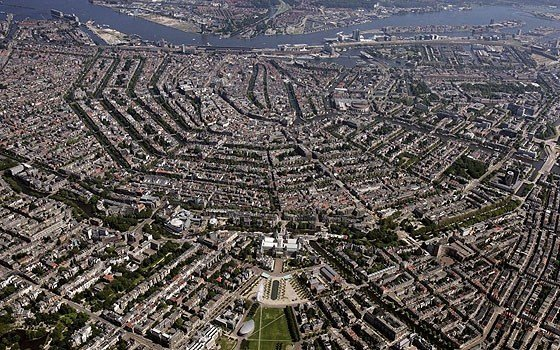
\includegraphics[width=4cm]{amsterdam.jpg}};
   \node[visible on=<2>] {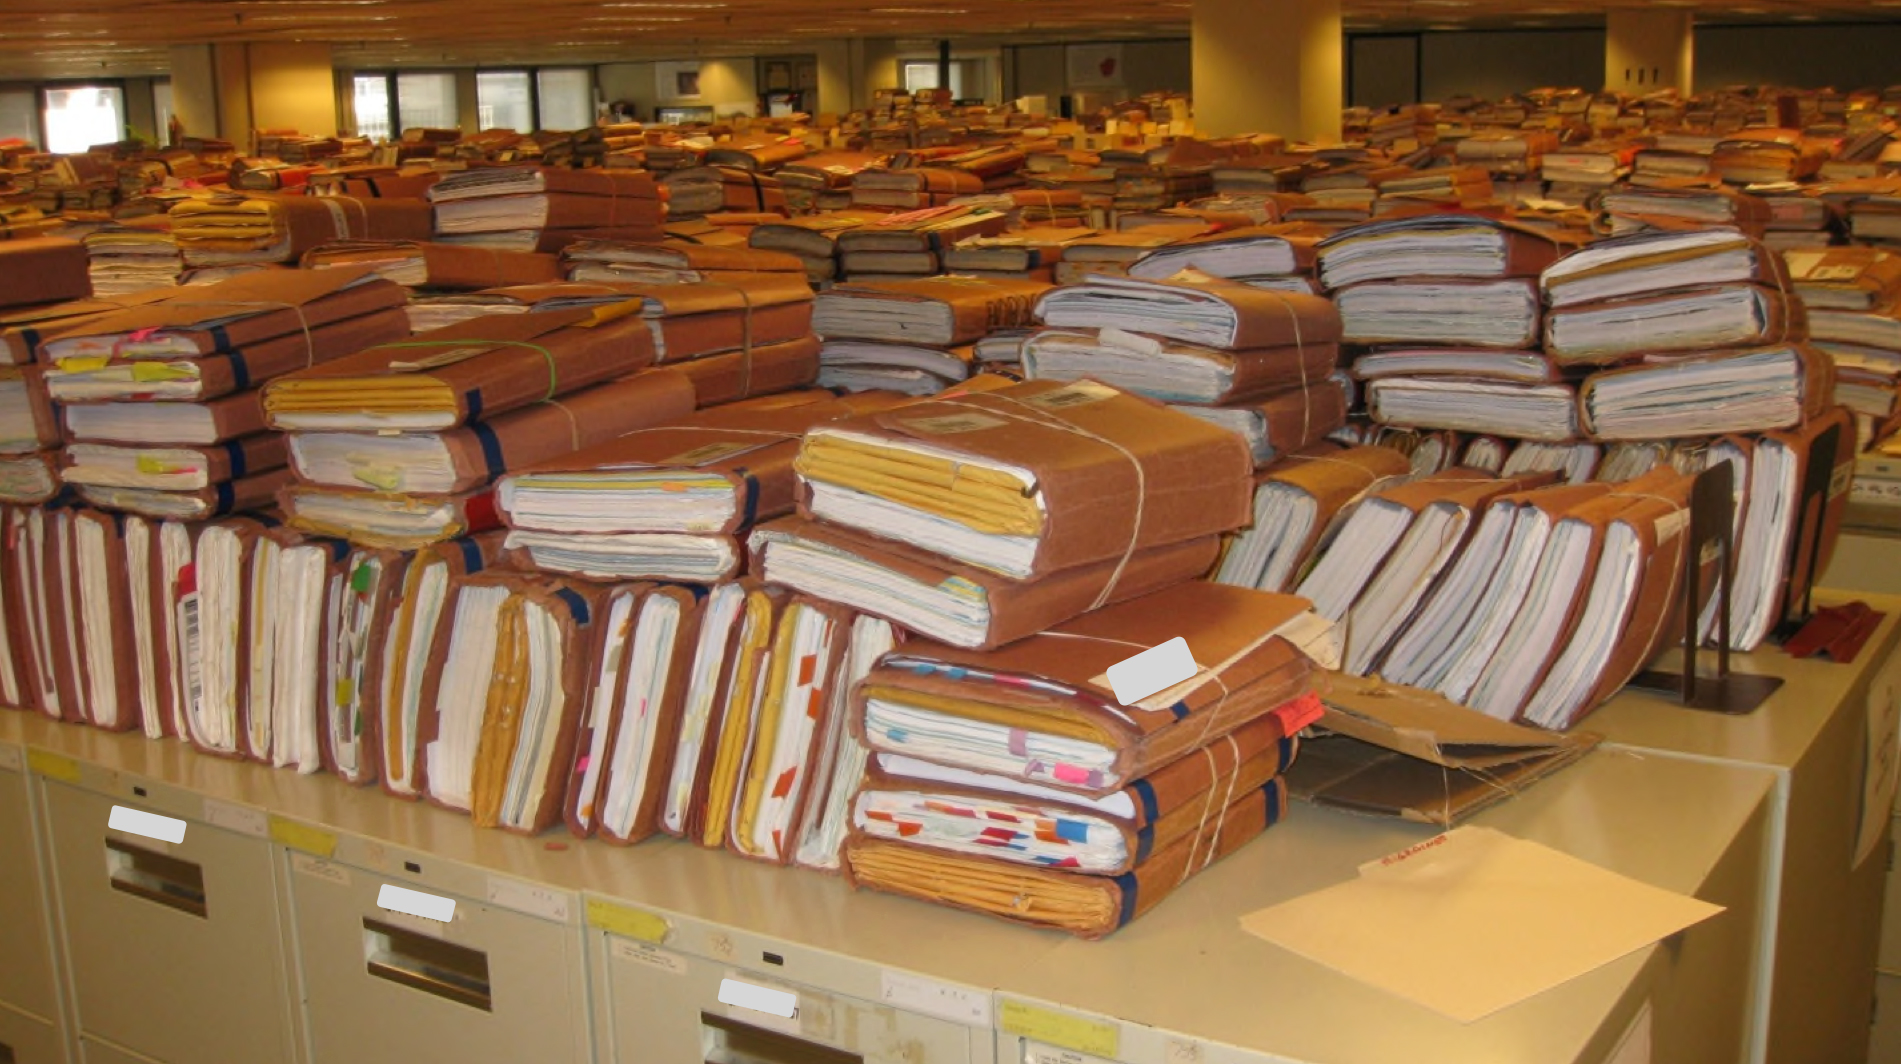
\includegraphics[width=4cm]{basementfiles.jpg}};
   \node[visible on=<3>] {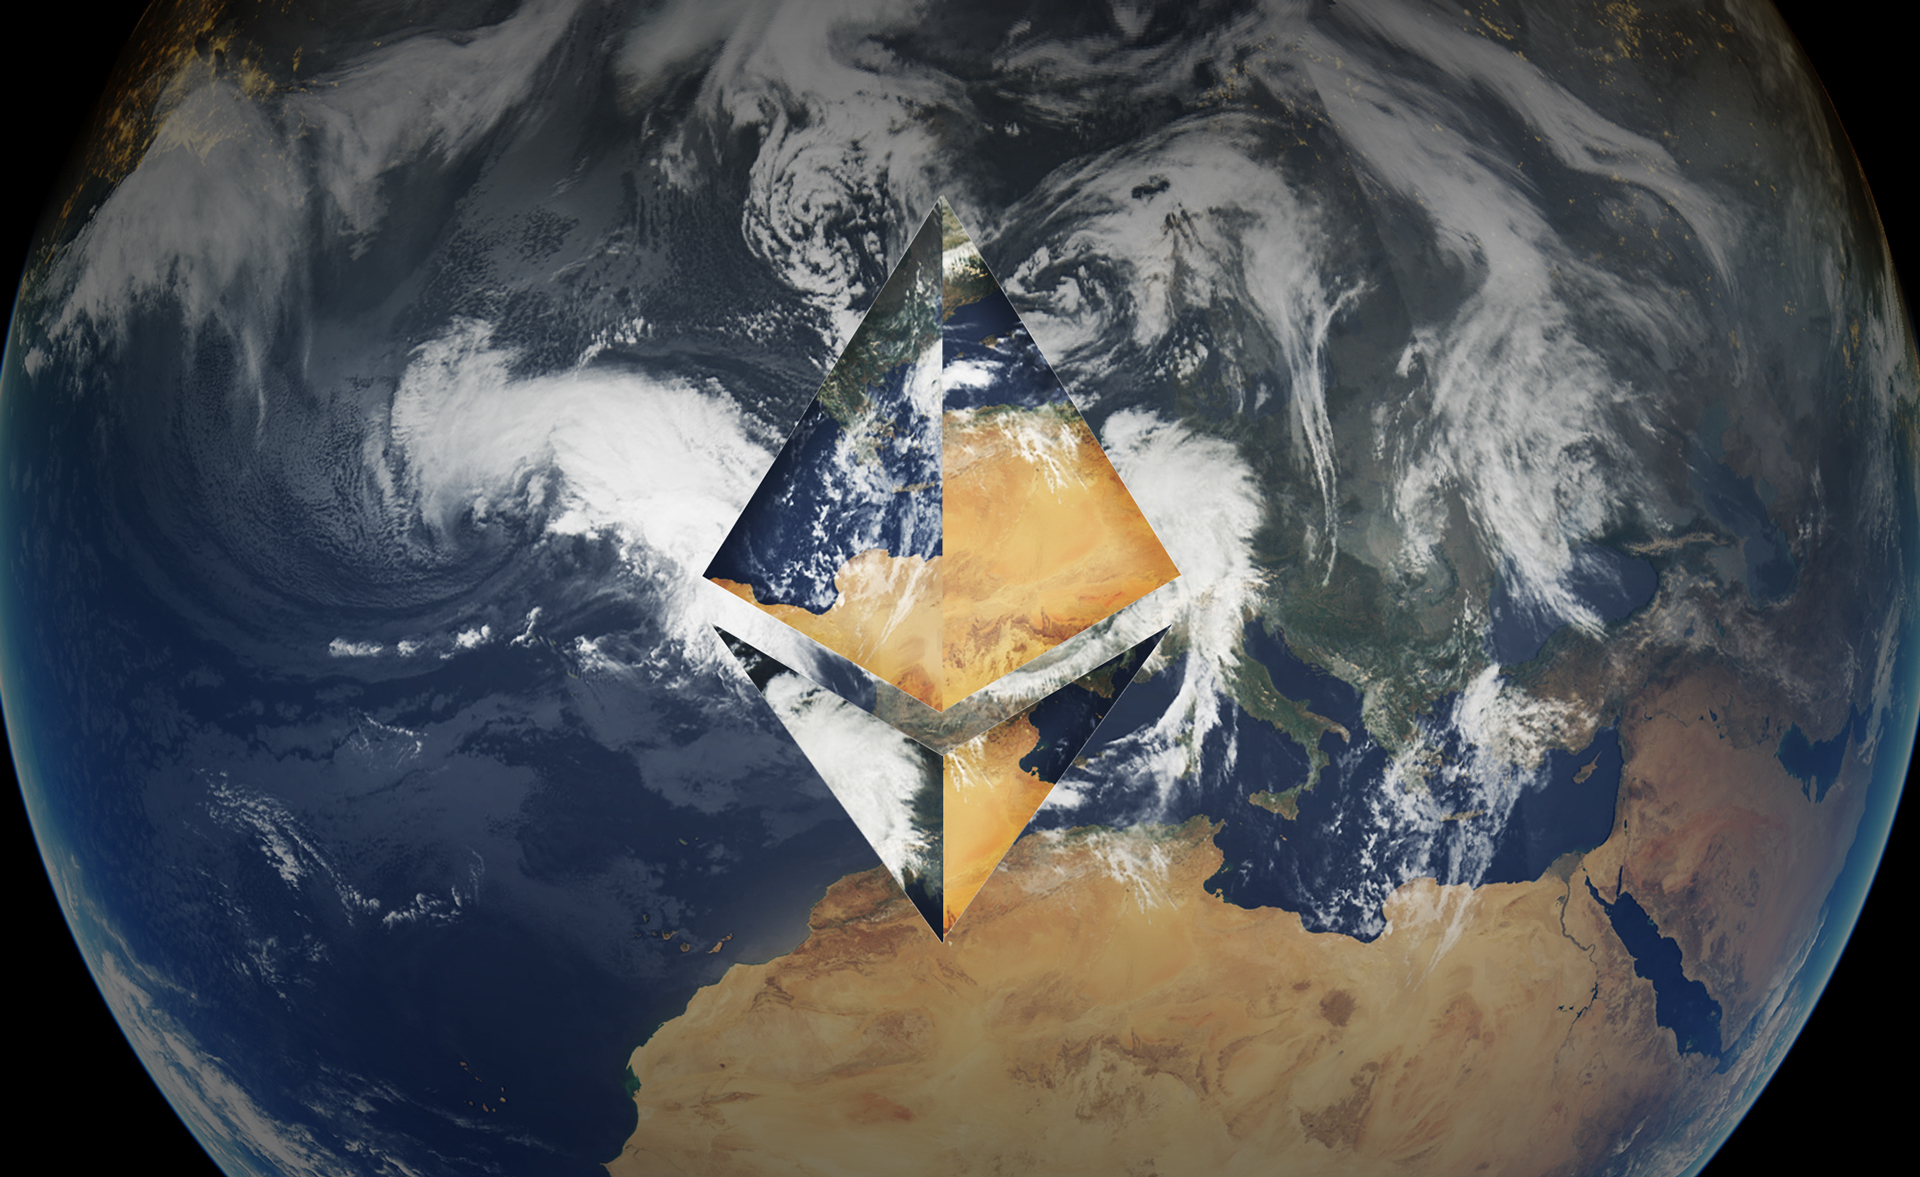
\includegraphics[width=4cm]{ethereumglobe.jpg}};
   \node[visible on=<4-6>] {
\includegraphics[width=4cm]{contract.jpg}};

  \end{tikzpicture}

 \end{column}

\end{columns}


 
\end{frame}

\wholeslide[So?]{What's so special about that?}

\begin{frame}{Why are smart contracts special?}

The contract is \alert<1>{self enforcing}.\\

\uncover<2->{
The money will be transferred if and only if the ownership of the apartment changes. In fact it is the transfer of ownership (as represented in the land registry) that releases the payment.\\}
\uncover<3->{
There is no need for a notary to hold on to the money (escrow) -- the contract itself can act as the trusted third pary.}
 
\end{frame}

\subsection{What else is there?}
\begin{frame}{What else can we do?}

For a start, anything that only really involves maintaining a database according to some rulues:
\begin{itemize}
 \item<2-> Domain Name System
 \item<3-> Money and bank accounts 
 \item<4-> Land registry
 \item<4-> ...
\end{itemize}

\uncover<4->{Also popular are interactions requiring only basic logic:}
\begin{itemize}
 \item<5-> Gambling and Betting
 \item<6-> Financial derivatives
 \item<7-> ``Fair" pyramid and Ponzi schemes
\end{itemize}

\end{frame}

\wholeslide{}

\section[examples]{Real-world examples}

\subsection[prediciton market]{The story of Intrade and Augur}
\begin{frame}{Intrade and Augur}

 Let me tell you the story of Intrade and Augur
 
\end{frame}

\subsection[bylaws]{Corporate bylaws}
\begin{frame}{bylaws on-chain}
We can imagine a company encoding all of its \textbf{corporate bylaws into smart contracts}. \\
For example the rules could say:
\begin{itemize}
 \item<2-> only the \textbf<2>{treasurer} can propose spending
 \item<3-> the proposed spending \textbf<3>{can only happen if} 3 board members agree...
 \item<4-> ...\textbf<4>{unless} it is more than 1000 Ether, in which case two-thirds must agree.
 \item<5-> There will be an \textbf<5>{election} for treasurer \textbf<5>{every year} on 1st September.
\end{itemize}
\uncover<6->{...and so on. Can be arbitrarily complex. It's up to you.}
\end{frame}
\begin{frame}{Benefits:}
When doing things this way, you are protected from some forms of corruption and you do not have to rely on weak legal systems to enforce the laws for you.
\begin{block}<2->{Lesson:}
 smart contracts are stubborn.
\end{block}

\uncover<3->{This means that they will execute as written.\:}
\uncover<4->{If you encode term limits, there will be term limits(*),}
\uncover<5->{if you code for monthly elections \alert<5>{there absolutely will be} monthly elections.}
 
\end{frame}

\subsection[crowdfunding]{Crowdfunding}
\begin{frame}{Crowdfunding and so on...}
 This technology allows people to \textbf{cooperate} and \textbf{coordinate} without needing to trust each other. People can pool resources and work towards common goals.
 \begin{itemize}
  \item Crowdfunding
  \item Voting and collective decision making.
  \item Governance and resource management.
 \end{itemize}
Because the \textit{logic} and the \textit{value} (currency) live on the same platform, incentives can be neatly modulated towards some goal.
\end{frame}



\subsection[copyright]{A story about copyright and DRM}
\begin{frame}{Copyright the right way?}
The story of micropayments.
\begin{block}<2->{Question}
Can we combine the act of listening to music with automatic (micro-)payments to the correct people? 
\end{block}
\begin{itemize}
 \item<3->{Payment-split: when paying for a song the money is channeled to \textit{all} the right people? \uncover<4->{\textbf{Yes.}}}
 \item<5->{Paying for every single listen? \uncover<6->{\textbf{No}. Scalability issues.}}
 \item<7->{Music file storage and distribution on ethereum blockchain? \uncover<8->{\textbf{No!} Ethereum may be a global computer, but it is slow and expensive. Good for smart contracts but not for data storage.} }
\end{itemize}

\end{frame}

\wholeslide{We need to look at how this all works under the hood.}

\section[tech]{A brief tour of the technology}

\subsection[blockchain]{The blockchain and proof-of-work}
\begin{frame}{Blockchain and proof-of-work}
 \only<1>{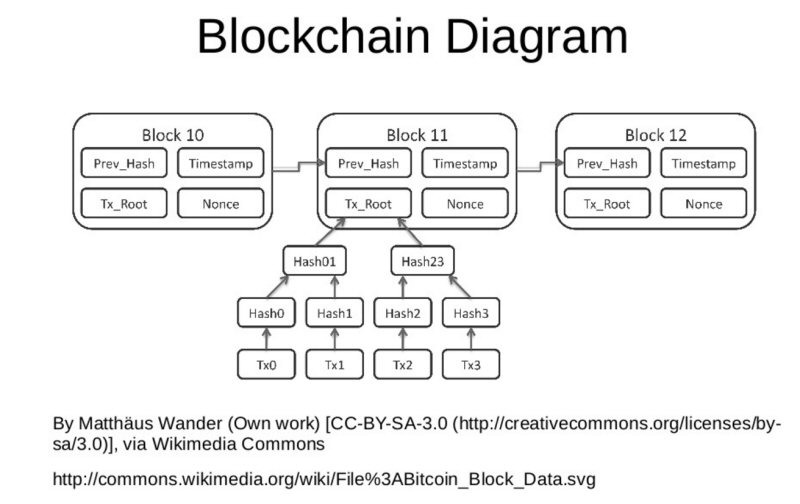
\includegraphics[width=9cm]{blockchain_diagram.jpg}}
 \only<2>{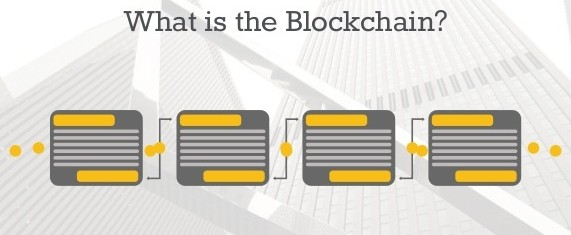
\includegraphics[width=9cm]{blockchain_diagram2.jpg}}
\end{frame}

\subsection[turing]{Turing-completness}
\begin{frame}{Ethereum is Turing complete}
 Ethereum is \textit{the} general purpose blockchain.\\[5mm]
 \textbf{Q:} What \alt<1>{information is stored in the blockchain?}{is contained in the transactions?}
 

   \begin{itemize}
  \item[Bitcoin] \alt<1>{Account balances}{Transfer}
  \item[Litecoin] \alt<1>{Account balances}{Transfer}
  \item[Dogecoin] \alt<1>{Account balances}{Transfer}
  \item[Ethereum] \alt<1>{Data of any complexity}{Computation of arbitrary(*) complexity}
 \end{itemize}
\uncover<2>{ }

 \end{frame}

 \wholeslide{So what about movies? music? chat? email?}
 
\subsection[data]{Swarm}
\begin{frame}{Swarm}
Swarm is a peer-to-peer file storage and distribution network integrated with ethereum.
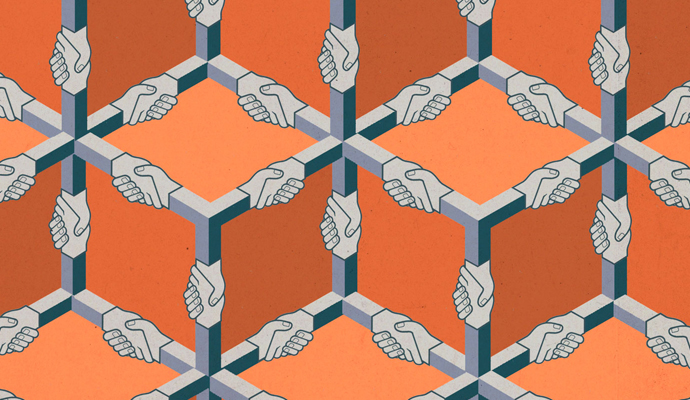
\includegraphics[width=8cm]{peerhandshake.jpg}
\end{frame}
% \subsection[talk]{Whisper}
% \begin{frame}{Whisper}
% Whisper is 
% 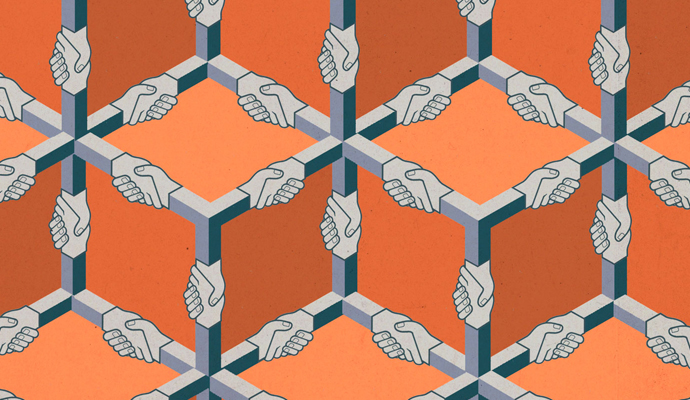
\includegraphics[width=8cm]{peerhandshake.jpg}
% \end{frame}

\section[web3]{The Web3 Vision}
\begin{frame}{The ethereum ecosystem}
\begin{columns}[T]
 \column{.3\textwidth}
  
\includegraphics[width=3cm]{ethereum.jpg}
 
\column{.3\textwidth}
  
\includegraphics[width=3cm]{swarm.jpg}

 \column{.3\textwidth}
  
\includegraphics[width=3cm]{whisper.jpg}
\end{columns}

 
\end{frame}

\begin{frame}{Web3}
\begin{center}

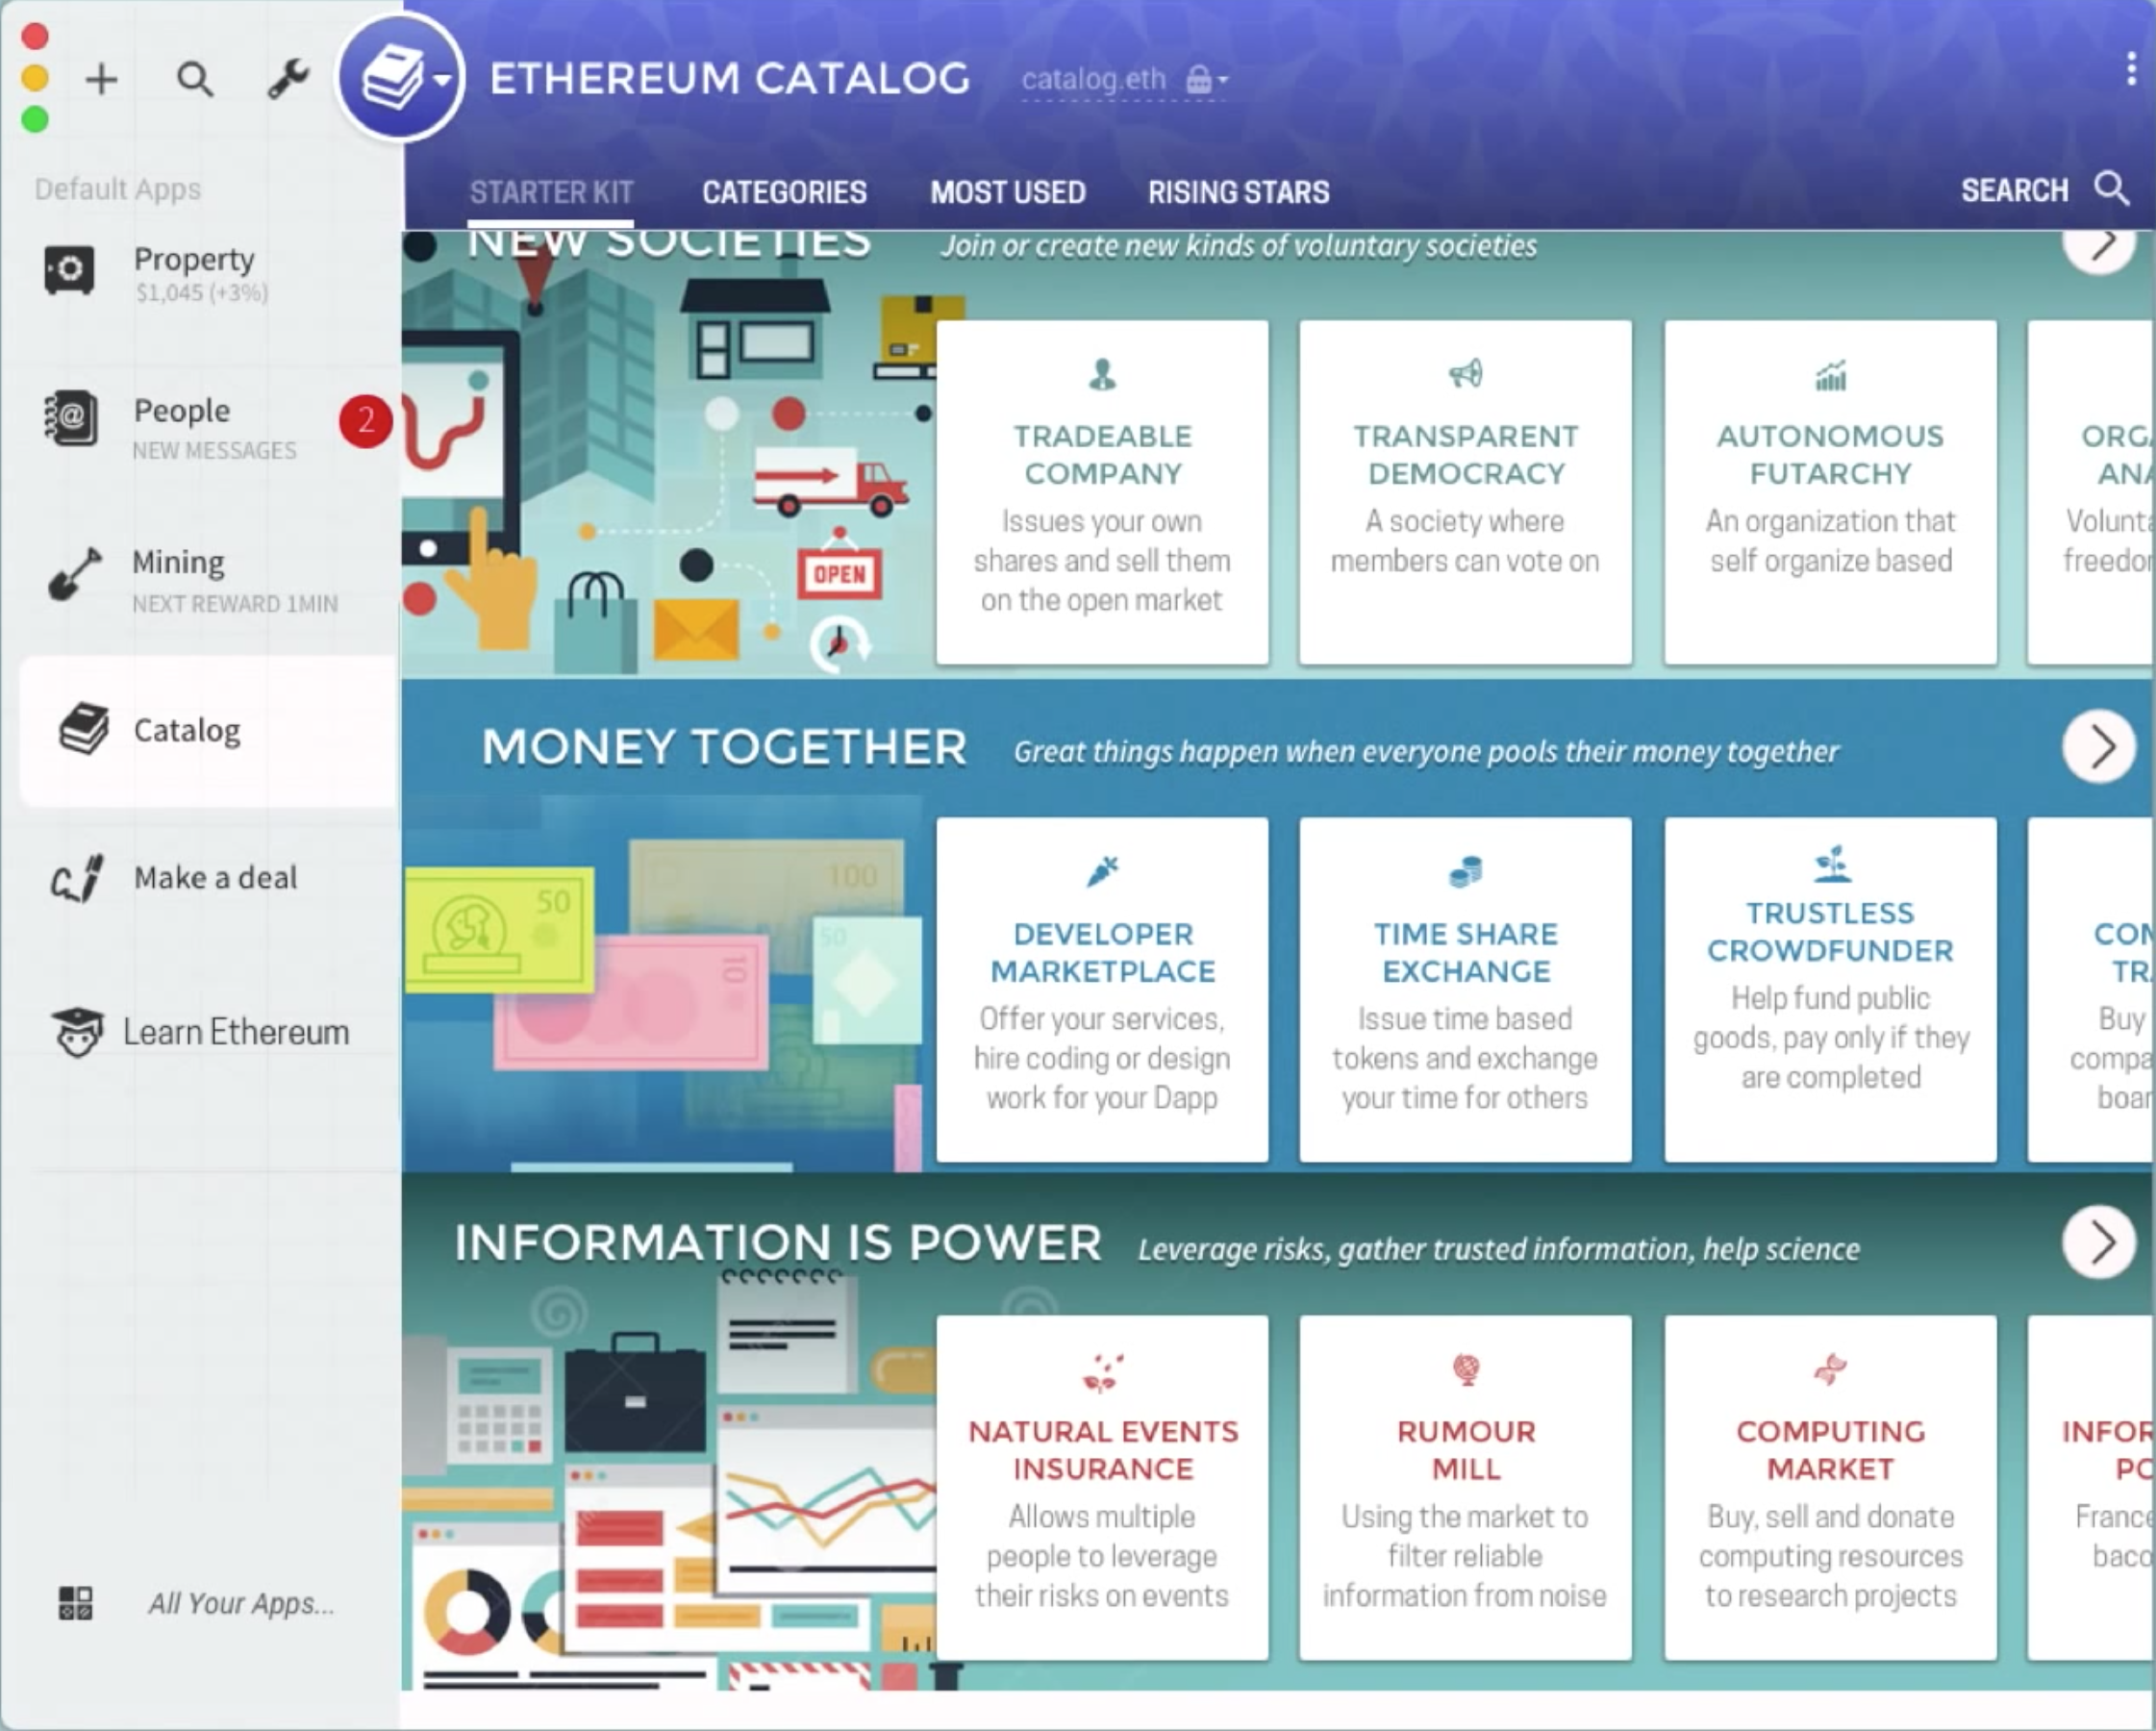
\includegraphics[width=8cm]{mistvision.png} 
 
\end{center}
\end{frame}



 
\end{document}
